%!TEX root=finmath1.tex
\part{Непрерывное время}
\chapter{Случайные процессы. Броуновское движение}
\label{ch:processes}
\chaptertoc

Дальнейшая часть курс будет посвящена моделям рынков с непрерывным временем и, главным образом, модели Блэка--Шоулса.
В связи с этим нам потребуется на некоторое время (на три лекции) погрузиться в теорию случайных процессов.

\section{Основные понятия, относящиеся к случайным процессам}

В этом разделе присутствует ряд технических определений и результатов (они отмечены звездочками).
Для практических применений они не так полезны, но, чтобы сохранить строгость изложения, мы их все-таки приводим.
При первом чтении их можно пропустить.

\begin{definition}
\emph{Случайный процесс $X$} "--- это семейство случайных величин $(X_t)_{t\ge 0}$, определенных на одном вероятностном пространстве $(\Omega,\F,\P)$.
\end{definition}

Время идет непрерывно, т.е.\ запись $t\ge0$ означает $t\in[0,\infty)$.
Мы также будем рассматривать случай конечного горизонта времени $t\in[0,T]$.

\begin{definition}
\emph{Траекторией} случайного процесса $X$, соответствующей случайному исходу $\omega$, называется функция $t\mapsto X_t(\omega)$.

Случайный процесс называется \emph{непрерывным}, если все траектории непрерывны.
Аналогично определяются процессы непрерывные слева или справа, неубывающие или невозрастающие, и \td
\end{definition}

\begin{definition}[$*$]
Случайный процесс $X$ называется \emph{измеримым}, если он измерим по паре переменных $(\omega,t)$, \te\ отображение $X(\omega,t)\colon\Omega\times\R_+ \to \R$ является $\F\otimes\B(\R_+)/\B(\R)$-измеримым.
\end{definition}

Далее мы будем считать, что все рассматриваемые процессы измеримы.
Свойство измеримости будет нужно, например, для определения интеграла по броуновскому движению в лекции \ref{ch:ito-integral}, а также в ряде других мест.
Следующее предложение дает простое достаточное условие измеримости, которое будет выполнено для большинства процессов, встречающихся далее в курсе.

\begin{proposition}[$*$]
Если случайный процесс $X$ непрерывен слева или непрерывен справа, то он измерим.
\end{proposition}

\begin{proof}
Непрерывный слева процесс $X$ можно приблизить кусочно"=постоянными процессами $X^n(\omega,t) = X(\omega, [nt]/n)$, \te\ для всех $t$ и $\omega$
\[
\lim_{n\to\infty} X^n(\omega,t) = X(\omega,t).
\]
Нетрудно проверить, что кусочно-постоянные процессы измеримы. Тогда $X$ измерим как предел измеримых отображений $X^n$.
Аналогично для непрерывных слева процессов.
\end{proof}

Следующее определение вводит понятие равенства случайных процессов.
(Полезно вспомнить, что для случайных величин вводят как минимум два понятия равенства: почти наверное и по распределению.)

\begin{definition}
Случайные процессы $X$ и $Y$ называются
\begin{itemize}
\item \emph{неразличимыми}, если у них \as\ совпадают траектории, \te\ $\P(\omega: X_t(\omega) = Y_t(\omega)\allowbreak \text{ для всех $t$}) = 1$;
\item \emph{эквивалентными}, если $X_t = Y_t$ \as\ для всех $t$ (синоним: $X$ является \emph{модификацией} $Y$);
\item \emph{одинаково распределенными}, если у них совпадают все конечномерные распределения, \te\ $(X_{t_1},\dots,X_{t_n}) = (Y_{t_1},\dots,Y_{t_n})$ по распределению для любых моментов времени $t_1,\dots,t_n$.
\end{itemize}
В этих определениях предполагается, что интервалы времени, на которых заданы оба процесса, одинаковы.
В определении неразличимости и эквивалентности считается, что процессы заданы на одном вероятностном пространстве.
\end{definition}

\begin{proposition}
Если процессы $X$ и $Y$ неразличимы, то они эквивалентны.
Если процессы $X$ и $Y$ непрерывны слева или непрерывны справа, то они неразличимы тогда и только тогда, когда они эквивалентны. 
\end{proposition}

\begin{proof}[Доказательство $(*)$]
Событие $\{\omega: X_t(\omega) \neq Y_t(\omega)\}$ является подмножеством события $\{\omega: X_t(\omega) \neq Y_t(\omega)\ \text{для некоторого $t$}\}$.
Поэтому если второе имеет нулевую вероятность, то и первое тоже.
Значит, из неразличимости следует эквивалентность.

Пусть теперь процессы $X$ и $Y$ непрерывны слева и эквивалентны (для непрерывных справа доказательство аналогично).
Воспользуемся тем, что любая непрерывная слева функция на $\R_+$ определяется по своим значениям на множестве неотрицательных рациональных чисел.
Тогда
\[
\{\omega: X_t(\omega) = Y_t(\omega)\ \text{для всех}\ t\}
= \bigcap_{t\in\mathbb{Q}_+} \{\omega: X_t(\omega) = Y_t(\omega)\}.
\]
В правой части берется пересечение счетного числа множеств.
Поэтому если каждое из этих множества имеет вероятность 1, то и пересечение имеет вероятность~1.
Следовательно, эквивалентность влечет неразличимость.
\end{proof}

Далее будем предполагать, что вероятностное пространство снабжено \emph{фильтрацией} $\FF=(\F_t)_{t\ge0}$, \te\ семейством $\sigma$-алгебр $\F_t$ таких, что $\F_s \subseteq \F_t$ для всех $s\le t$.
Аналогично определяется фильтрация для конечного горизонта времени. 

\begin{definition}
Случайный процесс $X$ называется \emph{согласованным с фильтрацией $\FF$}, если для каждого $t$ случайная величина $X_t$ является $\F_t$-измеримой.
\end{definition}

\begin{definition}
Фильтрацией, \emph{порожденной} процессом $X$ (или \emph{естественной фильтрацией} процесса $X$) называется семейство $\sigma$-алгебр $\F_t = \sigma(X_s,\ s\le t)$, \te\ $\F_t$ "--- это наименьшая $\sigma$-алгебра, относительно которой измеримы случайные величины $X_s$ для всех $s \le t$.
\end{definition}

\begin{remark}
Любой процесс согласован со своей естественной фильтрацией.
\end{remark}

\begin{remark}[$*$]
Для случайных последовательностей мы ввели еще понятие предсказуемости: величины $X_t$ должны быть измеримы относительно $\F_{t-1}$.
Соответствующее определение для случайных процессов более деликатно%
\footnote{Определение такое: процесс $X$ \emph{предсказуем}, если отображение $X(\omega,t)$ измеримо относительно \emph{предсказуемой $\sigma$-алгебры $\mathcal{P}$} на $\Omega\times\R_+$, которая по определению порождается всеми непрерывными согласованными процессами.},
так как в непрерывном времени нет <<предыдущего момента времени>>.
В этом курсе понятие предсказуемости нам не потребуется, хотя оно и играет важную роль в финансовой математике для общих моделей рынка в непрерывном времени.
\end{remark}

Следующее условие необходимо в разных технических результатах теории случайных процессов\footnote{Например, в теореме о существовании непрерывной справа и имеющей пределы слева модификации произвольного мартингала (см.~\cite{BulinskiShiryaev04}, стр.~142)}.
В финансовой математике можно считать его всегда выполненным, так как это не уменьшает общности рассуждений.

\begin{definition}[$*$]
Говорят, что фильтрованное вероятностное пространство $(\Omega,\F,\FF,\P)$ удовлетворяет \emph{обычным условиям}, если
\begin{alphenum}
\item вероятностное пространство $(\Omega,\F,\P)$ \emph{полно}, \te\ если событие $A\in\F$ имеет нулевую вероятность, то $B\in\F$ для любого подмножества $B\subseteq A$;
\item $\F_0$ содержит все события из $\F$ нулевой вероятности;
\item фильтрация $\FF$ непрерывна справа, \te\ $\F_t = \bigcap_{s>t} \F_s$ для всех $t\ge0$.
\end{alphenum}
\end{definition}


\section{Броуновское движение}
\subsection{Определение}

\begin{definition}
\emph{Броуновским движением} (или \emph{винеровским процессом}) на фильтрованном вероятностном пространстве $(\Omega,\F,\FF,\P)$ называется случайный процесс $W=(W_t)_{t\ge0}$ со следующими свойствами:
\begin{enumerate}
\item $W_0=0$ п.н.;
\item для любых $0\le s<t$ приращение $W_t-W_s$ не зависит от $\F_s$;
\item $W_t-W_s$ имеет нормальное распределение с математическим ожиданием 0 и дисперсией $t-s$, \te\ $W_t-W_s\sim N(0,t-s)$;
\item траектории $W$ непрерывны.
\end{enumerate}
\end{definition}

\begin{remark}
\begin{enumerate}
\item Из определения следует, что $W_t=W_t-W_0\sim N(0,t)$. 

\item Если фильтрация не указывается, то обычно имеется ввиду, что броуновское движение задано относительно своей естественной фильтрации.

\item Используя теорему Колмогорова о непрерывной модификации, можно показать, что если процесс $W$ удовлетворяет свойствам 1--3, то у него существует непрерывная модификация.
По этой причине условие непрерывности траекторий часто не включают в определение.

\item В литературе также часто используется символ $B$ для обозначения броуновского движения (B "--- Brownian, W "--- Wiener). У нас он будет занят под обозначение цены безрискового актива.
\end{enumerate}
\end{remark}

\begin{proposition}
Для любых моментов времени $0\le t_1<\dots<t_n$ случайный вектор $\xi = (W_{t_1}, \ldots, W_{t_n})$ имеет многомерное нормальное распределение со средним $\E W_{t_i} = 0$ и ковариацией $\cov(W_{t_i}, W_{t_j}) = \min(t_i,t_j)$.
\end{proposition}

\begin{proof}
Вектор $\zeta = (W_{t_1}, W_{t_2} - W_{t_1}, \ldots, W_{t_n} - W_{t_{n-1}})$ имеет нормальное распределение в силу того, что его компоненты нормально распределены и независимы. 
Вектор $\xi$ можно получить из $\zeta$ с помощью линейного преобразования, а именно
\[
W_{t_i} = \sum_{j=1}^i (W_{t_j} - W_{t_{j-1}}) + W_{t_1}.
\]
Следовательно, $\xi$ тоже имеет нормальное распределение. 
Кроме того, $\E W_{t_i} = \E (W_{t_i} - W_{0}) = 0$, и для любых $i < j$
\begin{multline*}
\cov(W_{t_i}, W_{t_j}) = E(W_{t_i}W_{t_j}) = \E (W_{t_i}(W_{t_j} - W_{t_i} + W_{t_i})) \\
= \E (W_{t_i}W_{t_i}) + \E (W_{t_i}(W_{t_j} - W_{t_i})) = t_i + 0 = t_i.
\end{multline*}
\end{proof}

\begin{remark}
Напомним, что многомерное нормальное распределение однозначно задается своим вектором средних и ковариационной матрицей.
Таким образом, предыдущее предложение характеризует конечномерные распределения броуновского движения.

Случайный процесс, у которого все конечномерные распределения являются нормальными, называется \emph{гауссовским процессом}.
Подобно многомерному нормальному распределению, гауссовский процесс характеризуется своей функцией среднего $\mu(t) = \E X_t$ и ковариационной функцией $\sigma(s,t) = \cov(X_s,S_t)$.
Это дает эквивалентное определение броуновского движения, которое часто встречается в литературе: это непрерывный гауссовский процесс с нулевым средним и ковариационной функцией $\sigma(s,t) = \min(s,t)$.
\end{remark}

На рис.~\ref{6:trajectory} показано, как выглядят типичные траектории броуновского движения.
Видно, что они устроены весьма хаотично и нерегулярно.
Следующее предложение содержит хорошо известные свойства траекторий броуновского движения. 
Доказательство можно найти во многих учебниках по случайным процессам (см., например, гл.~III в \cite{BulinskiShiryaev04}).

\begin{proposition}
С вероятностью 1 траектории броуновского движения не дифференцируемы ни в одной точке, не имеют точек роста и убывания, а также имеют бесконечную вариацию на любом отрезке $[a,b]$, где $a<b$.
\end{proposition}

\begin{figure}[h]
\centering
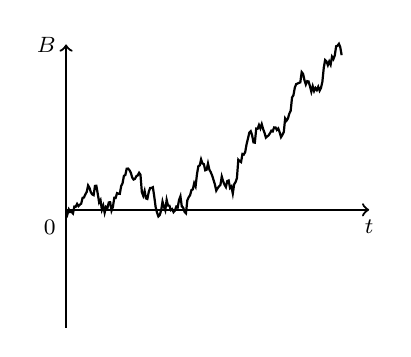
\begin{tikzpicture}[xscale=3.5]
\draw[thick,->] (0,0) node[below left] {\footnotesize $0$} -- (1.1,0) node[below] {\footnotesize $t$};
\draw[thick,->] (0,-1.5) -- (0,2.1) node[left] {\footnotesize $B$};
\draw[thick] (0.000,0.000)--(0.005,-0.056)--(0.010,0.004)--(0.015,-0.029)--(0.020,-0.027)--(0.025,-0.046)--(0.030,0.041)--(0.035,0.039)--(0.040,0.075)--(0.045,0.047)--(0.050,0.065)--(0.055,0.079)--(0.060,0.152)--(0.065,0.157)--(0.070,0.197)--(0.075,0.227)--(0.080,0.309)--(0.085,0.279)--(0.090,0.223)--(0.095,0.196)--(0.100,0.187)--(0.105,0.304)--(0.110,0.305)--(0.115,0.203)--(0.120,0.094)--(0.125,0.124)--(0.130,0.002)--(0.135,0.053)--(0.140,-0.036)--(0.145,0.036)--(0.150,0.019)--(0.155,0.094)--(0.160,0.096)--(0.165,-0.010)--(0.170,0.038)--(0.175,0.153)--(0.180,0.151)--(0.185,0.212)--(0.190,0.205)--(0.195,0.203)--(0.200,0.301)--(0.205,0.338)--(0.210,0.432)--(0.215,0.441)--(0.220,0.522)--(0.225,0.524)--(0.230,0.504)--(0.235,0.471)--(0.240,0.411)--(0.245,0.385)--(0.250,0.394)--(0.255,0.427)--(0.260,0.436)--(0.265,0.470)--(0.270,0.445)--(0.275,0.226)--(0.280,0.179)--(0.285,0.240)--(0.290,0.145)--(0.295,0.138)--(0.300,0.227)--(0.305,0.277)--(0.310,0.278)--(0.315,0.287)--(0.320,0.169)--(0.325,0.035)--(0.330,-0.034)--(0.335,-0.084)--(0.340,-0.065)--(0.345,-0.007)--(0.350,0.104)--(0.355,0.038)--(0.360,-0.007)--(0.365,0.126)--(0.370,0.054)--(0.375,0.053)--(0.380,-0.003)--(0.385,0.009)--(0.390,-0.029)--(0.395,-0.009)--(0.400,0.040)--(0.405,0.029)--(0.410,0.125)--(0.415,0.172)--(0.420,0.043)--(0.425,0.028)--(0.430,-0.027)--(0.435,-0.044)--(0.440,0.120)--(0.445,0.160)--(0.450,0.185)--(0.455,0.251)--(0.460,0.260)--(0.465,0.339)--(0.470,0.299)--(0.475,0.451)--(0.480,0.554)--(0.485,0.564)--(0.490,0.641)--(0.495,0.589)--(0.500,0.580)--(0.505,0.502)--(0.510,0.509)--(0.515,0.588)--(0.520,0.510)--(0.525,0.478)--(0.530,0.436)--(0.535,0.381)--(0.540,0.323)--(0.545,0.244)--(0.550,0.275)--(0.555,0.298)--(0.560,0.316)--(0.565,0.422)--(0.570,0.362)--(0.575,0.319)--(0.580,0.289)--(0.585,0.365)--(0.590,0.372)--(0.595,0.278)--(0.600,0.298)--(0.605,0.208)--(0.610,0.324)--(0.615,0.352)--(0.620,0.402)--(0.625,0.636)--(0.630,0.617)--(0.635,0.606)--(0.640,0.709)--(0.645,0.702)--(0.650,0.734)--(0.655,0.832)--(0.660,0.905)--(0.665,0.981)--(0.670,0.999)--(0.675,0.949)--(0.680,0.857)--(0.685,0.853)--(0.690,1.031)--(0.695,1.029)--(0.700,1.077)--(0.705,1.034)--(0.710,1.088)--(0.715,1.026)--(0.720,0.980)--(0.725,0.917)--(0.730,0.932)--(0.735,0.946)--(0.740,0.973)--(0.745,1.005)--(0.750,0.996)--(0.755,1.047)--(0.760,1.046)--(0.765,1.014)--(0.770,1.033)--(0.775,0.986)--(0.780,0.923)--(0.785,0.951)--(0.790,0.987)--(0.795,1.160)--(0.800,1.133)--(0.805,1.159)--(0.810,1.221)--(0.815,1.257)--(0.820,1.427)--(0.825,1.454)--(0.830,1.552)--(0.835,1.596)--(0.840,1.604)--(0.845,1.612)--(0.850,1.619)--(0.855,1.749)--(0.860,1.727)--(0.865,1.647)--(0.870,1.592)--(0.875,1.634)--(0.880,1.630)--(0.885,1.570)--(0.890,1.500)--(0.895,1.569)--(0.900,1.509)--(0.905,1.547)--(0.910,1.521)--(0.915,1.562)--(0.920,1.513)--(0.925,1.549)--(0.930,1.625)--(0.935,1.801)--(0.940,1.902)--(0.945,1.885)--(0.950,1.837)--(0.955,1.884)--(0.960,1.844)--(0.965,1.944)--(0.970,1.914)--(0.975,1.960)--(0.980,2.077)--(0.985,2.084)--(0.990,2.108)--(0.995,2.064)--(1.000,1.964);

\end{tikzpicture}
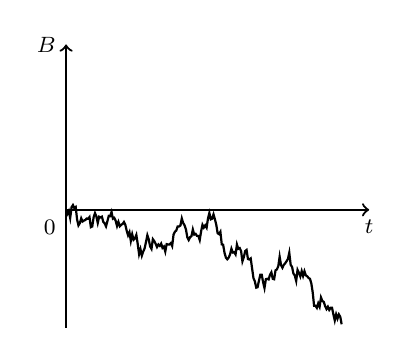
\begin{tikzpicture}[xscale=3.5]
\draw[thick,->] (0,0) node[below left] {\footnotesize $0$} -- (1.1,0) node[below] {\footnotesize $t$};
\draw[thick,->] (0,-1.5) -- (0,2.1) node[left] {\footnotesize $B$};
\draw[thick] (0.000,0.000)--(0.005,-0.051)--(0.010,-0.015)--(0.015,-0.103)--(0.020,0.033)--(0.025,0.060)--(0.030,0.022)--(0.035,0.036)--(0.040,-0.122)--(0.045,-0.198)--(0.050,-0.169)--(0.055,-0.108)--(0.060,-0.148)--(0.065,-0.136)--(0.070,-0.129)--(0.075,-0.111)--(0.080,-0.114)--(0.085,-0.092)--(0.090,-0.220)--(0.095,-0.212)--(0.100,-0.096)--(0.105,-0.042)--(0.110,-0.084)--(0.115,-0.166)--(0.120,-0.088)--(0.125,-0.097)--(0.130,-0.087)--(0.135,-0.152)--(0.140,-0.173)--(0.145,-0.210)--(0.150,-0.145)--(0.155,-0.077)--(0.160,-0.080)--(0.165,-0.028)--(0.170,-0.112)--(0.175,-0.102)--(0.180,-0.139)--(0.185,-0.206)--(0.190,-0.154)--(0.195,-0.209)--(0.200,-0.190)--(0.205,-0.181)--(0.210,-0.155)--(0.215,-0.189)--(0.220,-0.265)--(0.225,-0.324)--(0.230,-0.284)--(0.235,-0.395)--(0.240,-0.311)--(0.245,-0.380)--(0.250,-0.363)--(0.255,-0.319)--(0.260,-0.433)--(0.265,-0.563)--(0.270,-0.500)--(0.275,-0.582)--(0.280,-0.530)--(0.285,-0.491)--(0.290,-0.409)--(0.295,-0.323)--(0.300,-0.376)--(0.305,-0.464)--(0.310,-0.496)--(0.315,-0.373)--(0.320,-0.397)--(0.325,-0.431)--(0.330,-0.473)--(0.335,-0.440)--(0.340,-0.458)--(0.345,-0.429)--(0.350,-0.483)--(0.355,-0.466)--(0.360,-0.530)--(0.365,-0.436)--(0.370,-0.440)--(0.375,-0.440)--(0.380,-0.423)--(0.385,-0.460)--(0.390,-0.314)--(0.395,-0.278)--(0.400,-0.262)--(0.405,-0.211)--(0.410,-0.211)--(0.415,-0.199)--(0.420,-0.110)--(0.425,-0.169)--(0.430,-0.196)--(0.435,-0.249)--(0.440,-0.349)--(0.445,-0.383)--(0.450,-0.347)--(0.455,-0.335)--(0.460,-0.250)--(0.465,-0.314)--(0.470,-0.305)--(0.475,-0.331)--(0.480,-0.331)--(0.485,-0.383)--(0.490,-0.275)--(0.495,-0.190)--(0.500,-0.225)--(0.505,-0.197)--(0.510,-0.227)--(0.515,-0.110)--(0.520,-0.041)--(0.525,-0.121)--(0.530,-0.113)--(0.535,-0.058)--(0.540,-0.118)--(0.545,-0.188)--(0.550,-0.297)--(0.555,-0.309)--(0.560,-0.279)--(0.565,-0.439)--(0.570,-0.443)--(0.575,-0.547)--(0.580,-0.607)--(0.585,-0.628)--(0.590,-0.608)--(0.595,-0.567)--(0.600,-0.494)--(0.605,-0.542)--(0.610,-0.537)--(0.615,-0.566)--(0.620,-0.441)--(0.625,-0.495)--(0.630,-0.486)--(0.635,-0.522)--(0.640,-0.655)--(0.645,-0.602)--(0.650,-0.524)--(0.655,-0.510)--(0.660,-0.625)--(0.665,-0.631)--(0.670,-0.617)--(0.675,-0.744)--(0.680,-0.867)--(0.685,-0.908)--(0.690,-0.988)--(0.695,-0.982)--(0.700,-0.899)--(0.705,-0.823)--(0.710,-0.823)--(0.715,-0.920)--(0.720,-0.993)--(0.725,-0.881)--(0.730,-0.876)--(0.735,-0.884)--(0.740,-0.825)--(0.745,-0.794)--(0.750,-0.876)--(0.755,-0.882)--(0.760,-0.769)--(0.765,-0.757)--(0.770,-0.716)--(0.775,-0.595)--(0.780,-0.702)--(0.785,-0.736)--(0.790,-0.700)--(0.795,-0.679)--(0.800,-0.653)--(0.805,-0.625)--(0.810,-0.545)--(0.815,-0.699)--(0.820,-0.724)--(0.825,-0.809)--(0.830,-0.835)--(0.835,-0.903)--(0.840,-0.763)--(0.845,-0.799)--(0.850,-0.846)--(0.855,-0.779)--(0.860,-0.840)--(0.865,-0.780)--(0.870,-0.832)--(0.875,-0.844)--(0.880,-0.866)--(0.885,-0.876)--(0.890,-0.935)--(0.895,-1.049)--(0.900,-1.219)--(0.905,-1.219)--(0.910,-1.245)--(0.915,-1.188)--(0.920,-1.231)--(0.925,-1.114)--(0.930,-1.157)--(0.935,-1.169)--(0.940,-1.223)--(0.945,-1.260)--(0.950,-1.231)--(0.955,-1.271)--(0.960,-1.244)--(0.965,-1.244)--(0.970,-1.327)--(0.975,-1.405)--(0.980,-1.328)--(0.985,-1.381)--(0.990,-1.329)--(0.995,-1.359)--(1.000,-1.454);

\end{tikzpicture}
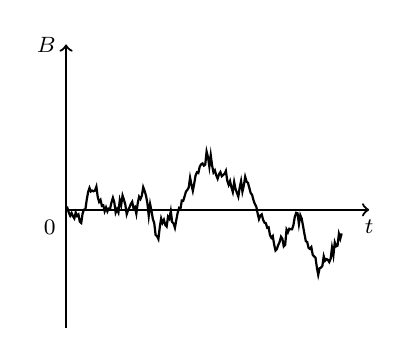
\begin{tikzpicture}[xscale=3.5]
\draw[thick,->] (0,0) node[below left] {\footnotesize $0$} -- (1.1,0) node[below] {\footnotesize $t$};
\draw[thick,->] (0,-1.5) -- (0,2.1) node[left] {\footnotesize $B$};
\draw[thick] (0.000,0.000)--(0.005,0.021)--(0.010,-0.036)--(0.015,-0.075)--(0.020,-0.041)--(0.025,-0.082)--(0.030,-0.109)--(0.035,-0.034)--(0.040,-0.078)--(0.045,-0.060)--(0.050,-0.152)--(0.055,-0.167)--(0.060,-0.047)--(0.065,0.002)--(0.070,0.002)--(0.075,0.128)--(0.080,0.225)--(0.085,0.278)--(0.090,0.233)--(0.095,0.244)--(0.100,0.235)--(0.105,0.244)--(0.110,0.294)--(0.115,0.162)--(0.120,0.101)--(0.125,0.126)--(0.130,0.051)--(0.135,0.058)--(0.140,-0.018)--(0.145,0.030)--(0.150,-0.020)--(0.155,0.018)--(0.160,0.019)--(0.165,0.095)--(0.170,0.153)--(0.175,0.097)--(0.180,-0.035)--(0.185,0.008)--(0.190,-0.033)--(0.195,0.124)--(0.200,0.061)--(0.205,0.181)--(0.210,0.127)--(0.215,0.067)--(0.220,-0.056)--(0.225,-0.005)--(0.230,0.029)--(0.235,0.074)--(0.240,0.102)--(0.245,0.014)--(0.250,0.034)--(0.255,-0.049)--(0.260,0.083)--(0.265,0.166)--(0.270,0.137)--(0.275,0.180)--(0.280,0.287)--(0.285,0.240)--(0.290,0.181)--(0.295,0.085)--(0.300,-0.076)--(0.305,0.071)--(0.310,-0.014)--(0.315,-0.117)--(0.320,-0.170)--(0.325,-0.321)--(0.330,-0.334)--(0.335,-0.371)--(0.340,-0.223)--(0.345,-0.110)--(0.350,-0.165)--(0.355,-0.127)--(0.360,-0.192)--(0.365,-0.212)--(0.370,-0.088)--(0.375,-0.114)--(0.380,-0.018)--(0.385,-0.155)--(0.390,-0.172)--(0.395,-0.228)--(0.400,-0.131)--(0.405,-0.038)--(0.410,0.022)--(0.415,0.009)--(0.420,0.118)--(0.425,0.114)--(0.430,0.169)--(0.435,0.231)--(0.440,0.252)--(0.445,0.283)--(0.450,0.408)--(0.455,0.318)--(0.460,0.241)--(0.465,0.332)--(0.470,0.437)--(0.475,0.476)--(0.480,0.467)--(0.485,0.548)--(0.490,0.577)--(0.495,0.589)--(0.500,0.561)--(0.505,0.574)--(0.510,0.740)--(0.515,0.670)--(0.520,0.549)--(0.525,0.694)--(0.530,0.561)--(0.535,0.475)--(0.540,0.501)--(0.545,0.437)--(0.550,0.395)--(0.555,0.452)--(0.560,0.479)--(0.565,0.427)--(0.570,0.443)--(0.575,0.457)--(0.580,0.494)--(0.585,0.368)--(0.590,0.317)--(0.595,0.365)--(0.600,0.287)--(0.605,0.227)--(0.610,0.352)--(0.615,0.263)--(0.620,0.216)--(0.625,0.167)--(0.630,0.282)--(0.635,0.364)--(0.640,0.231)--(0.645,0.308)--(0.650,0.419)--(0.655,0.359)--(0.660,0.343)--(0.665,0.279)--(0.670,0.212)--(0.675,0.191)--(0.680,0.124)--(0.685,0.074)--(0.690,0.043)--(0.695,-0.045)--(0.700,-0.118)--(0.705,-0.073)--(0.710,-0.058)--(0.715,-0.126)--(0.720,-0.164)--(0.725,-0.171)--(0.730,-0.229)--(0.735,-0.223)--(0.740,-0.323)--(0.745,-0.355)--(0.750,-0.333)--(0.755,-0.441)--(0.760,-0.517)--(0.765,-0.498)--(0.770,-0.446)--(0.775,-0.407)--(0.780,-0.342)--(0.785,-0.368)--(0.790,-0.464)--(0.795,-0.445)--(0.800,-0.252)--(0.805,-0.286)--(0.810,-0.240)--(0.815,-0.247)--(0.820,-0.247)--(0.825,-0.195)--(0.830,-0.089)--(0.835,-0.038)--(0.840,-0.044)--(0.845,-0.181)--(0.850,-0.069)--(0.855,-0.111)--(0.860,-0.208)--(0.865,-0.307)--(0.870,-0.397)--(0.875,-0.409)--(0.880,-0.484)--(0.885,-0.497)--(0.890,-0.474)--(0.895,-0.572)--(0.900,-0.591)--(0.905,-0.607)--(0.910,-0.731)--(0.915,-0.826)--(0.920,-0.742)--(0.925,-0.734)--(0.930,-0.713)--(0.935,-0.589)--(0.940,-0.646)--(0.945,-0.626)--(0.950,-0.634)--(0.955,-0.663)--(0.960,-0.622)--(0.965,-0.482)--(0.970,-0.579)--(0.975,-0.414)--(0.980,-0.464)--(0.985,-0.456)--(0.990,-0.307)--(0.995,-0.367)--(1.000,-0.300);

\end{tikzpicture}
\caption{Траектории броуновского движения.}
\label{6:trajectory}
\end{figure}


\subsection{Мартингальное и марковское свойства броуновского движения}

\begin{definition}
Случайный процесс $X$ называется \emph{мартингалом} относительно фильтрации $\FF$, если
\begin{alphenum}
\item он согласован с фильтрацией $\FF$;
\item $\E|X_t| < \infty$ для всех $t$;
\item $\E(X_t\mid\F_s) = X_s$ \as\ для всех $s\le t$.
\end{alphenum}
Если в последнем условии заменить равенство на неравенство $\ge$, то получим определение \emph{субмартингала}, а если на $\le$, то определение \emph{супермартингала}.
\end{definition}

\begin{proposition}
Броуновское движение является мартингалом.
\end{proposition}
\begin{proof}
Имеем
\[
\E(W_t\mid\F_s) = \E(W_t - W_s + W_s\mid\F_s) 
= W_s + \E(W_t - W_s) = W_s,
\]
где воспользовались тем, что приращение $W_t - W_s$ не зависит от $\F_s$ и имеет нулевое математическое ожидание.
\end{proof}

\begin{remark}
Точно так же доказывается, что любой процесс с независимыми приращениями и $\E X_t\equiv c$ является мартингалом.  
\end{remark}

\begin{definition}
Процесс $X$ называется \emph{марковским} относительно фильтрации $\FF$, если для любых $s\le t_1<\dots<t_n$ и борелевских множеств $A_1,\dots,A_n$ выполнено равенство%
\footnote{Условная вероятность события $B$ относительно $\sigma$-алгебры $\G$ определяется как условное математическое ожидание соответствующего индикатора: $\P(B\mid\G) = \E (I_B \mid \G)$.}
\begin{equation}
\label{5:markov}
\P(X_{t_1}\in A_1,\dots,X_{t_n}\in A_n\mid\F_s) = \P(X_{t_1}\in A_1,\dots,X_{t_n}\in A_n\mid X_s)\ \text{п.н.}
\end{equation}
\end{definition}

Смысл этого определения состоит в следующем: для того, чтобы знать условное распределение значений процесса в будущем (\te\ конечномерное распределение $(X_{t_1},\dots,X_{t_n})$), достаточно знать его значение в текущий момент времени $s$, но не нужно знать всю предыдущую информацию, содержащуюся в $\F_s$.

Эквивалентное определение марковского процесса можно получить, если заменить формулу \eqref{5:markov} на условие, что для любой функции $f$, удовлетворяющей условию $\E|f(X_{t_1},\dots,X_{t_n})|<\infty$, выполнено равенство
\[
\E(f(X_{t_1},\dots,X_{t_n})\mid\F_s) = \E(f(X_{t_1},\dots,X_{t_n})\mid X_s)\ \text{п.н.}
\]

Следующее определение дает удобное понятие для работы с условными распределениями марковского процесса.

\begin{definition}
\label{pr:markov-transition}
Функция $\P(s,x,t,A)$ с аргументами $0\le s \le t$, $x\in\R$, $A\in\B(\R)$ называется \emph{марковской переходной функцией}, если
\begin{alphenum}
\item при фиксированных $s,x,t$ функция $B\mapsto P(s,x,t,A)$ является вероятностной мерой на $\B(\R)$;
\item при фиксированных $s,t,A$ функция $x\mapsto P(s,x,t,A)$ измерима;
\item $\P(s,x,s,A) = \I(x\in A)$ для любых $s,x,A$;
\item для любого $u\in[s,t]$ выполнено \emph{уравнение Колмогорова"--~Чепмена}:
\[
P(s,x,t,A) = \int_\R P(u,y,t,A) P(s,x,u,\,dy).
\]
\end{alphenum}
Говорят, что марковский процесс $X$ обладает переходной функцией $\P(s,x,t,A)$, если $\P(X_t \in A\mid X_s = x) = \P(s,x,t,A)$ \as\ для всех $s,x,t,A$.
%\footnote{Напомним, что условное математическое ожидание $\E(X\mid Y)$ можно представить как функцию $g(Y)$.
%Тогда запись $\E(X\mid Y=y)$ обозначает значение $g(y)$; см.~лекцию \ref{ch:mart}.}
\end{definition}

Переходную функцию нужно понимать как вероятность того, что, начиная из точки $x$ в момент времени $s$, процесс попадет в множество $A$ в момент времени $t$.
Условия a) и b) в определении \ref{pr:markov-transition} "--- технические, они гарантируют, что переходная функция <<хорошо устроена>>.
Условие c) означает, что если $t=s$, то процесс <<никуда не уйдет>> за нулевое время.
Уравнение Колмогорова"--~Чепмена (условие d) имеет следующий смысл: вероятность перехода из точки $x$ в множество $A$ за время $[s,t]$ может быть найдена из вероятностей перехода из точки $x$ в промежуточную точку $y$ за время $[s,u]$ и из $y$ в множество $A$ за время $[u,t]$, где $y$ пробегает всевозможные значения.

Известно, что у любого марковского процесса со значениями в $\R$ (или в $\R^n$) переходная функция существует.

\begin{definition}
Марковская переходная функция (или соответствующий ей марковский процесс) называется \emph{однородной}, если она зависит только от разности $t-s$, \te\ $\P(s,x,t,A) = \P(0,x,t-s,A)$.
\end{definition}

\begin{definition}
Если для всех $s<t$ и $x$ переходная функция марковского процесса $X$ обладает плотностью $p(s,x,t,y)$, \te\ выполнено равенство
\[
\P(s,x,t,A) = \int_A p(s,x,t,y)\,dy,
\]
то функция $p(s,x,t,y)$ называется \emph{переходной плотностью} процесса $X$.
\end{definition}

\begin{proposition}
Броуновское движение является однородным марковским процессом с переходной плотностью
\[
p(s,x,t,y) = \frac{1}{\sqrt{2\pi(t-s)}}\exp\left(-\frac{(y-x)^2}{2(t-s)}\right).
\] 
\end{proposition}
\begin{remark}
Легко заметить, что $p(s,x,t,y)$ есть плотность нормального распределения со средним $x$ и дисперсией $t-s$.
\end{remark}
\begin{proof}
Марковское свойство следует из того, что приращения $W_{t_i}-W_s$ не зависят от $\F_s$ при $t_i>s$, и, следовательно%
\footnote{Здесь используется такой факт: если случайная величина $Y$ является $\G$-измеримой, а случайный вектор $X$ не зависит от $\G$, то $\E(f(X,Y) \mid \G) = g(Y)$, где $g(y) = \E(f(X,y))$.
Результат справедлив при условии, что $\E| f(X,Y)| < \infty$.}, 
\[
\E( f(W_{t_1}, \ldots, W_{t_n}) \mid \F_s)
= \E( f(W_{t_1} - W_s + W_s, \ldots, W_{t_n} - W_s + W_s) \mid \F_s)
= g(W_s),
\]
где $g(x) = \E f(W_{t_1} - W_s + x, \ldots, W_{t_n} - W_s + x)$.
Аналогично получаем
\[
\P(W_t \in B \mid W_s = x) = \P( W_t - W_s + x \in B),
\]
и тогда формула для переходной плотности следует из того, что $W_t - W_s$ имеет нормальное распределение с нулевым средним и дисперсией $t-s$.
\end{proof}


\section{Броуновское движение со сносом и геометрическое броуновское движение}

\begin{definition}
Броуновским движением с коэффициентом \emph{сноса} $\mu\in\R$, коэффициентом \emph{диффузии} $\sigma>0$ и начальным условием $x\in\R$ относительно фильтрации $\FF$ называется процесс
\[
X_t = x + \mu t + \sigma W_t,
\]
где $W$ "--- броуновское движение относительно $\FF$.

Иногда такой процесс называют \emph{общим броуновским движением} (или даже просто броуновским движением, а для $x=0$, $\mu=1$, $\sigma=1$ используют термин \emph{стандартное броуновское движение}).
\end{definition}

Следующий результат непосредственно вытекает из свойств стандартного броуновского движения.

\begin{proposition}
Общее броуновское движение является однородным марковским процессом.
Оно является мартингалом при $\mu=0$, субмартингалом при $\mu\ge0$ и супермартингалом при $\mu\le0$.
\end{proposition}

\begin{definition}
\emph{Геометрическим броуновским движением} с коэффициентом \emph{сноса} $\mu\in\R$, коэффициентом \emph{волатильности} $\sigma>0$ и начальным условием $s>0$ относительно фильтрации $\FF$ называется процесс
\[
S_t = s e^{\sigma W_t + (\mu-\frac{\sigma^2}{2})t},
\]
где $W$ "--- броуновское движение относительно $\FF$.
\end{definition}

Качественное отличие геометрического броуновского движения от обычного такое же как у мультипликативного случайного блуждания от аддитивного (см.~примеры в лекции~3).
В частности, у геометрического броуновского движения нормально распределены и независимы приращения его логарифма, а не самого процесса. 

Геометрическое броуновское движение будет играть важную роль в дальнейшем изложении.
В частности, оно задает цену рискового актива в модели \bs.

Отметим, что странный на первый взгляд член $-\frac{\sigma^2}{2}t$ в экспоненте вводится для того, чтобы сделать геометрическое броуновское движение мартингалом в случае $\mu=0$, как показывает следующее предложение.

\begin{proposition}
Геометрическое броуновское движение является однородным марковским процессом.
Оно является мартингалом при $\mu=0$, субмартингалом при $\mu\ge0$ и супермартингалом при $\mu\ge0$.
Кроме того, $\E S_t = s e^{\mu t}$.
\end{proposition}

\begin{proof}
Марковское свойство следует из того, что имеется взаимно"=однозначное соответствие между $S_t$ и $W_t$.
Мартингальное (или суб/супермартингальное) свойство следует из равенства
\[
\E (S_t \mid \F_u) = S_u \E(e^{(\mu-\frac{\sigma^2}{2})(t-u) + \sigma(W_t-W_u)}) = S_u e^{\mu(t-u)},
\]
где воспользовались тем, что $\E e^{\sigma (W_t-W_u)} = e^{\frac{\sigma^2}{2} (t-u)}$.
\end{proof}


\summary

\begin{itemize}
\item В этом курсе случайные процессы рассматриваются на фильтрованных вероятностных пространствах $(\Omega,\F,\FF,\P)$. Случайный процесс $
X$ называется согласованным с фильтрацией $\FF$, если для каждого $t$ случайная величина $X_t$ измерима относительно $\F_t$.

\item Определение броуновского движения: непрерывный случайный процесс с нулевым начальным значением и независимыми приращениями, которые имеют нормальное распределение со средним 0 и дисперсией $\D (W_t-W_s) = t-s$. Эквивалентное определение: непрерывный гауссовский процесс с нулевым средним и ковариационной функцией $\cov(W_t,W_s) = \min(s,t)$.

\item Броуновское движение является мартингалом и марковским процессом, у которого переходные вероятности задаются нормальным распределением.

\item Общее броуновское движение "--- это процесс $X_t = x + \mu t + \sigma W_t$.

\item Геометрическое броуновское движение "--- это процесс $S_t = s e^{\sigma W_t + (\mu-\frac{\sigma^2}{2})t}$. При $\mu=0$ он является мартингалом.
\end{itemize}
